\documentclass{beamer}
\setbeamertemplate{frametitle}[default][center]
%Information to be included in the title page:
\title{\Large\textbf{Dydaktyczny symulator wybranych rozwiązań warstwy fizycznej sieci Ethernet}}
\author{Michał Iwanicki, Mateusz Bauer, Marcin Garnowski}
\institute{Politechnika Gdańska}
\date{2023}

\begin{document}

\frame{\titlepage}

\begin{frame}
\frametitle{Uruchamianie}
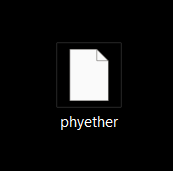
\includegraphics[width=0.25\textwidth]{images/prezentacja_start1.png}
\hfill
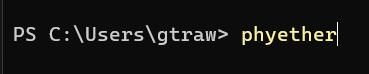
\includegraphics[width=0.65\textwidth]{images/prezentacja_start2.png}
\end{frame}

\begin{frame}
\frametitle{Poruszanie się po symulatorze}

\includegraphics[width=0.95\textwidth]{images/zakladki.png}
\end{frame}

\begin{frame}
\frametitle{Reed-Solomon}
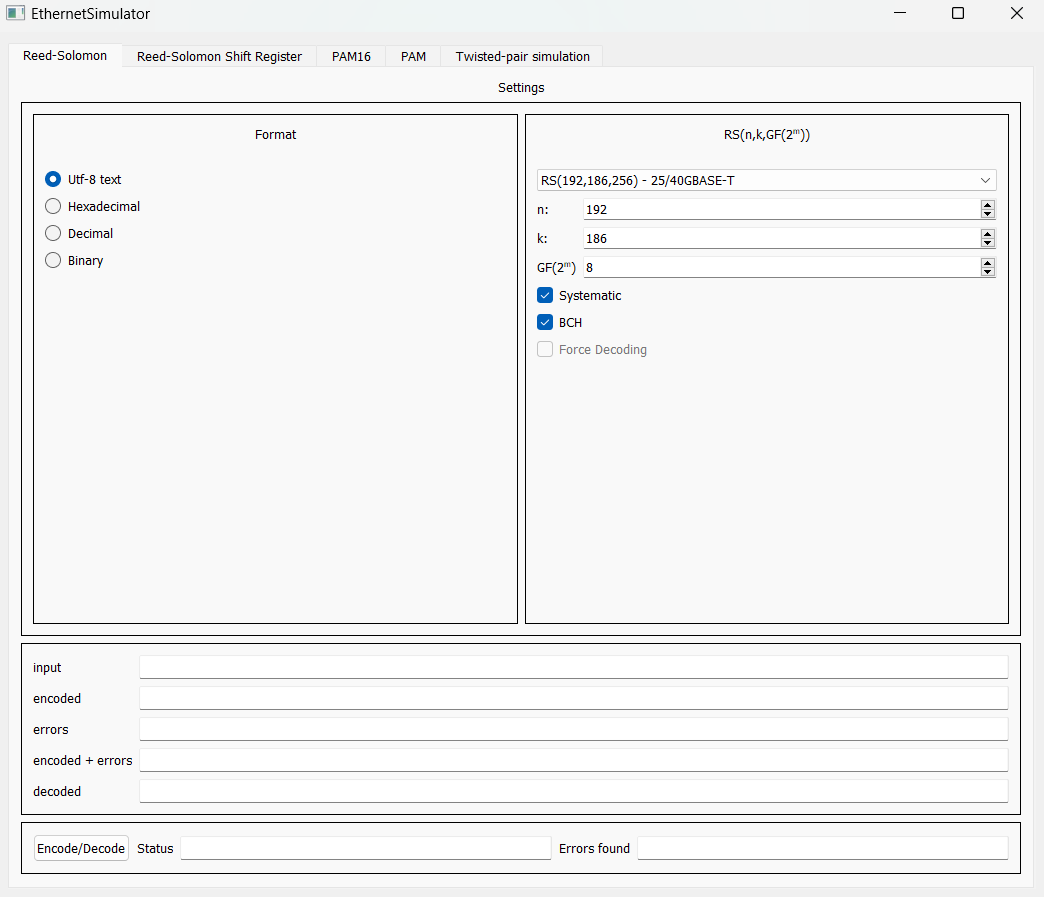
\includegraphics[width=0.95\textwidth]{images/prezentacja_rs.png}
\end{frame}

\begin{frame}
\frametitle{Reed-Solomon Shift Register}
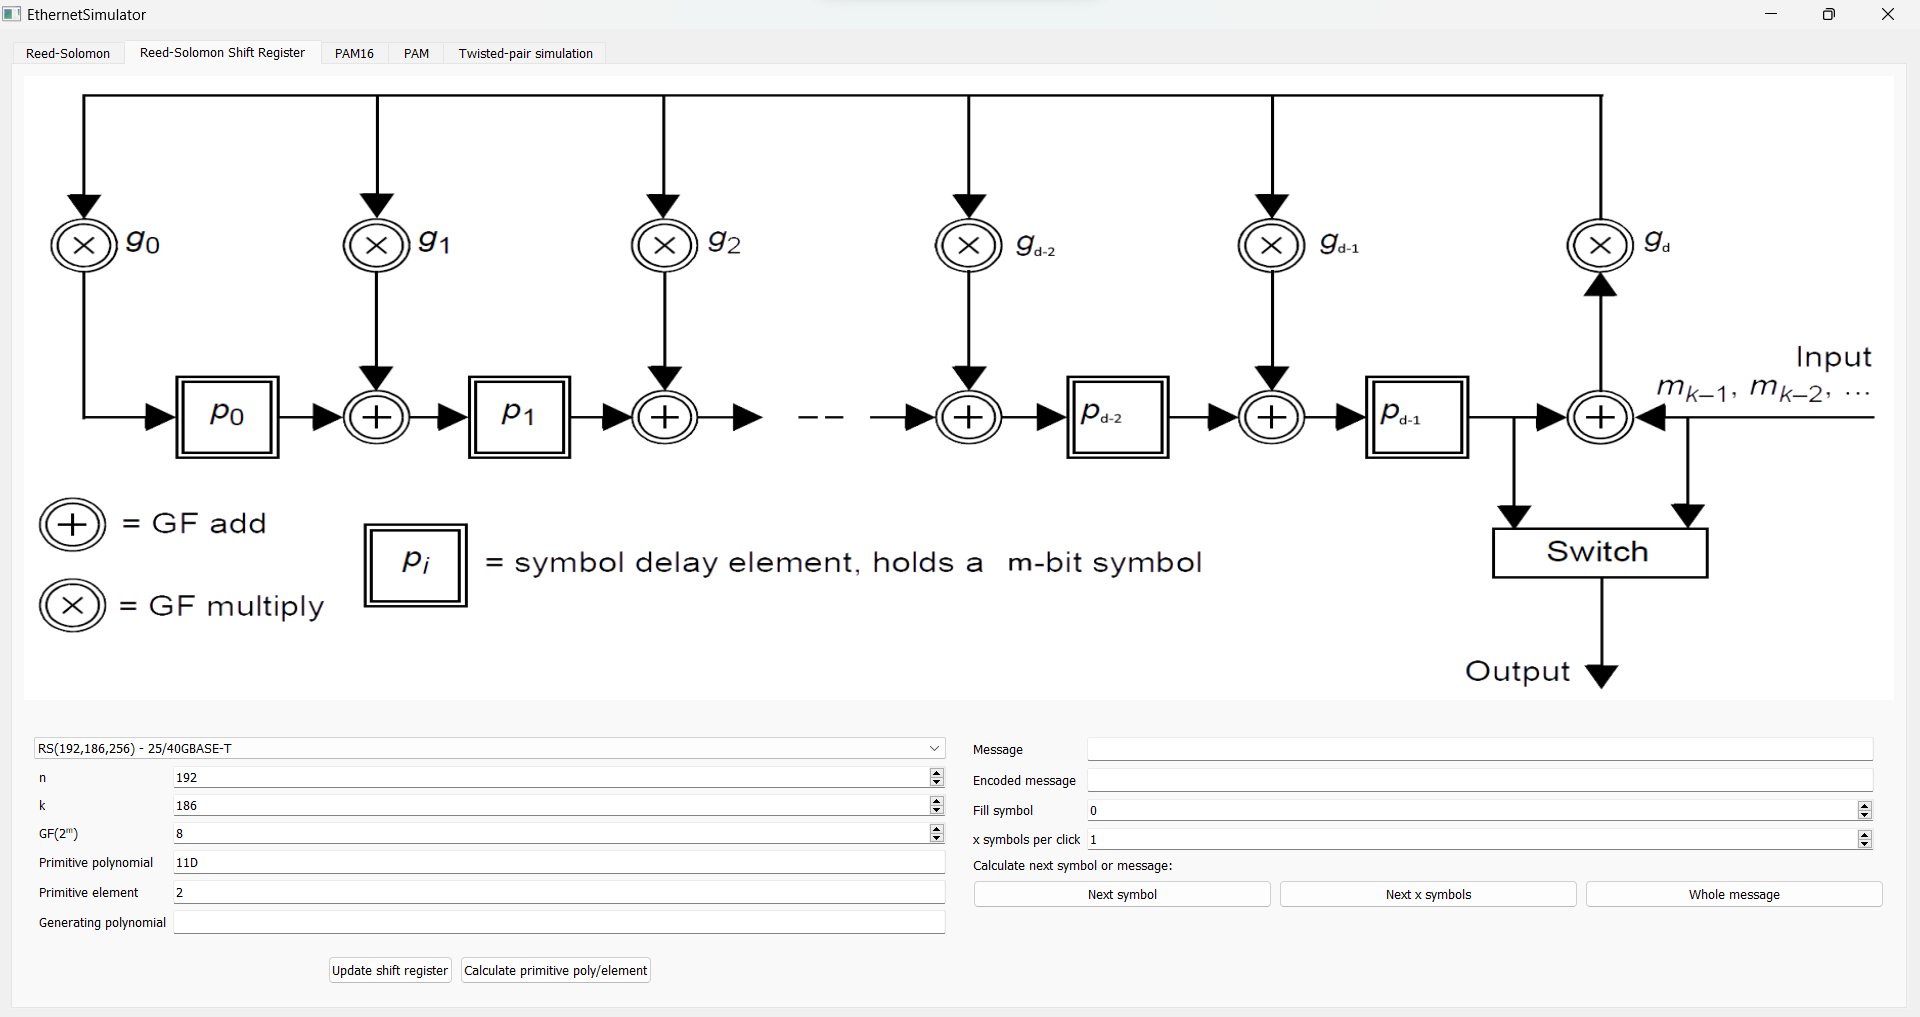
\includegraphics[width=0.95\textwidth]{images/prezentacja_rs_sr.png}
\end{frame}

\begin{frame}
\frametitle{PAM16}
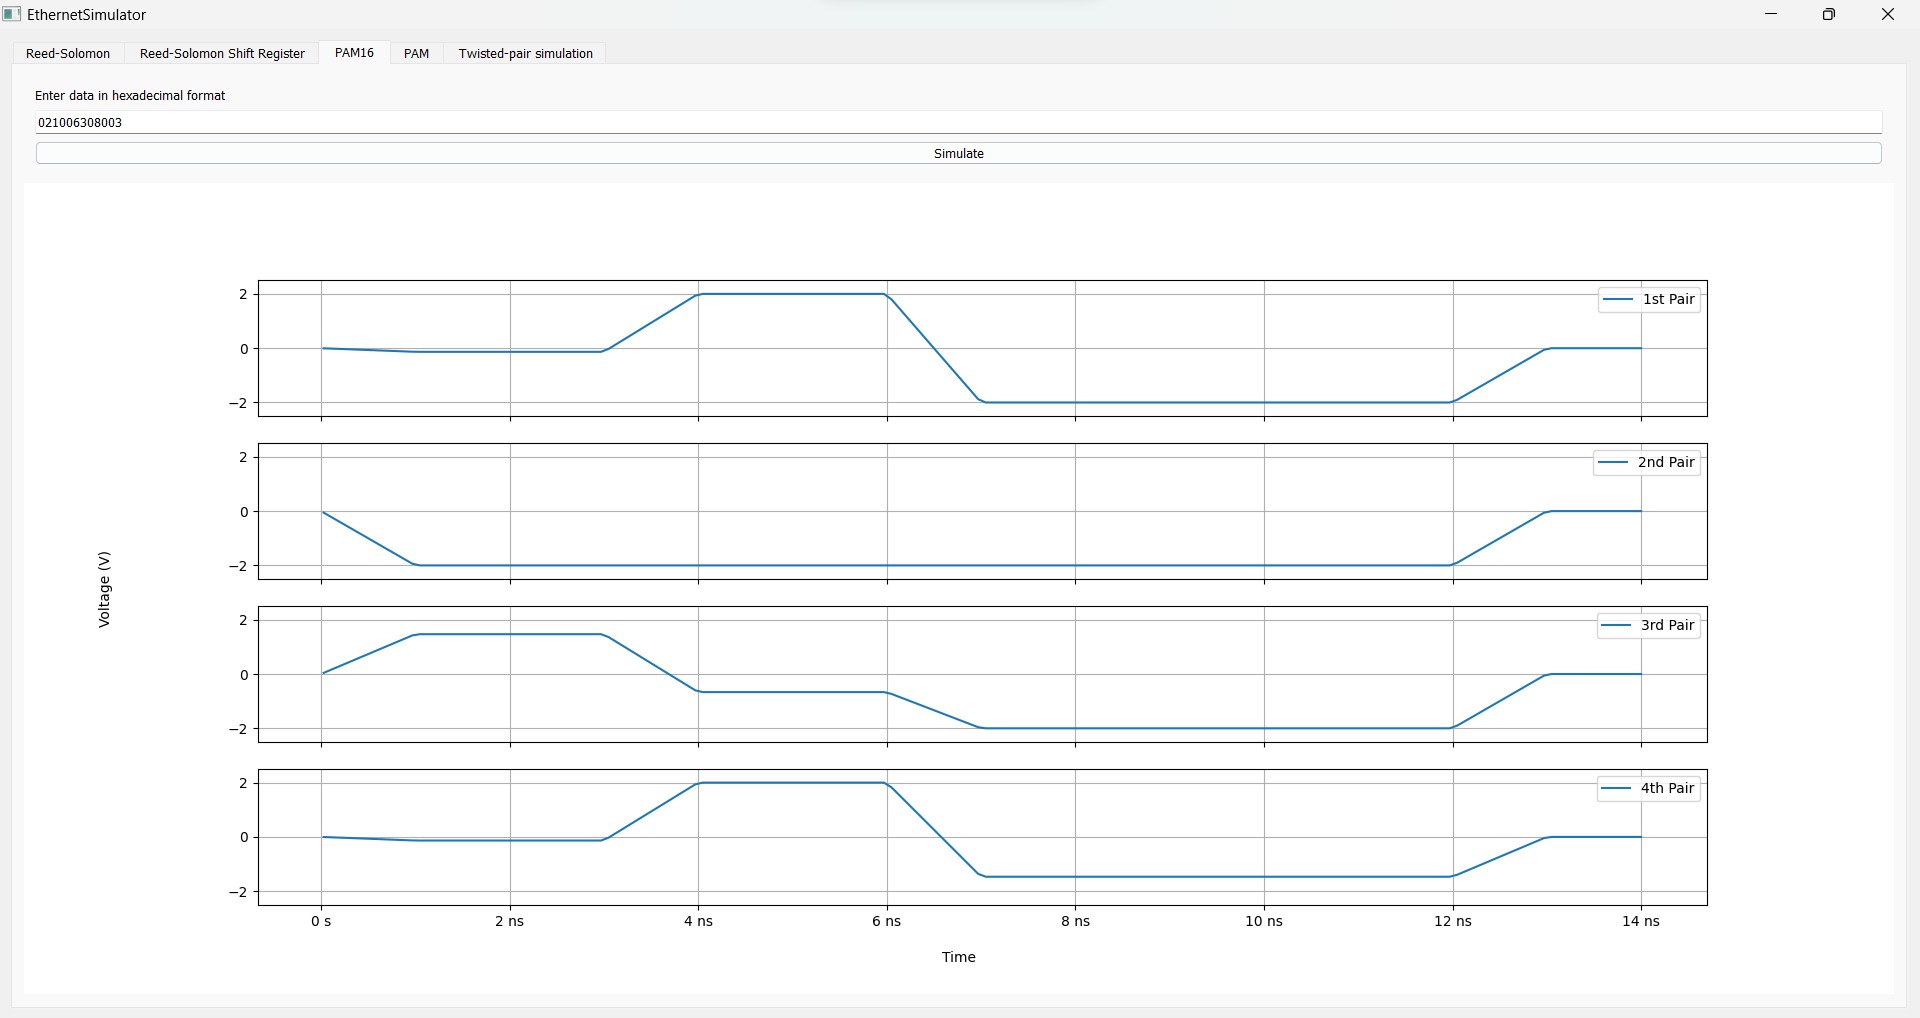
\includegraphics[width=0.95\textwidth]{images/prezentacja_pam16.png}
\end{frame}

\begin{frame}
\frametitle{PAM}
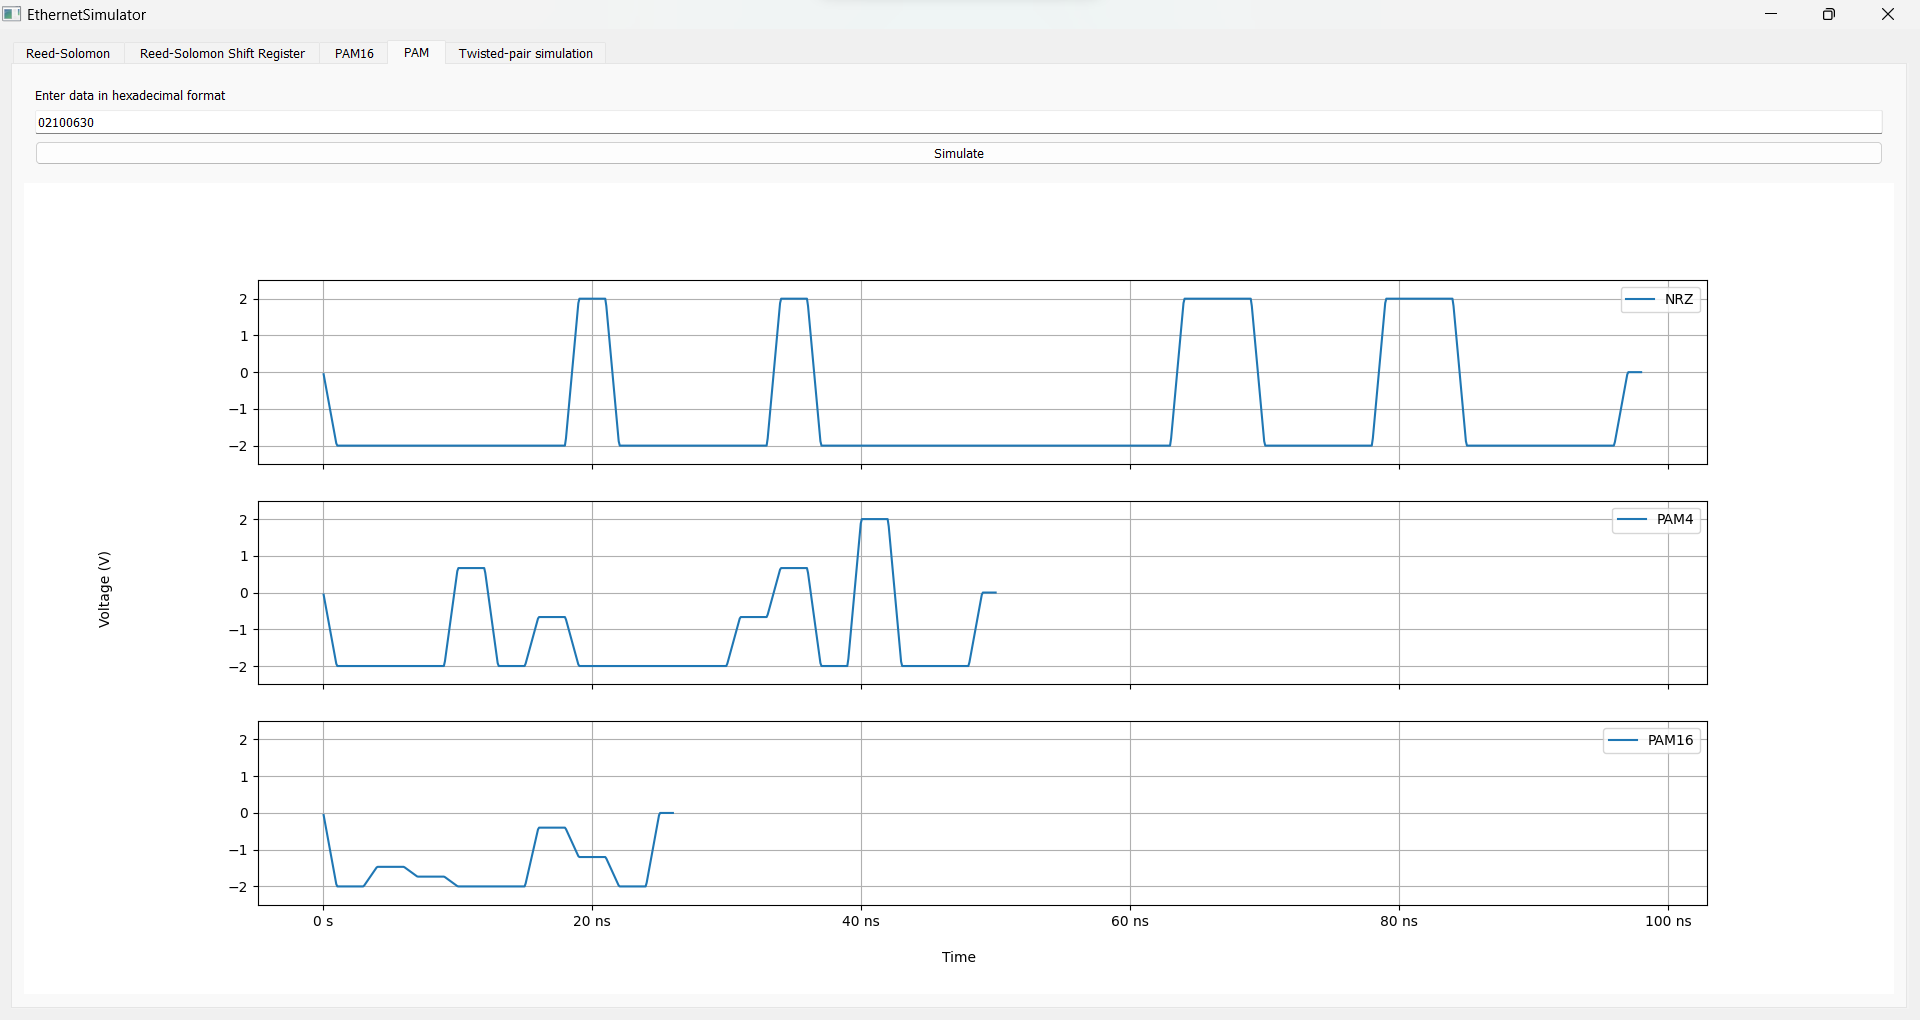
\includegraphics[width=0.95\textwidth]{images/prezentacja_pam.png}
\end{frame}

\begin{frame}
\frametitle{Twisted-pair simulation}
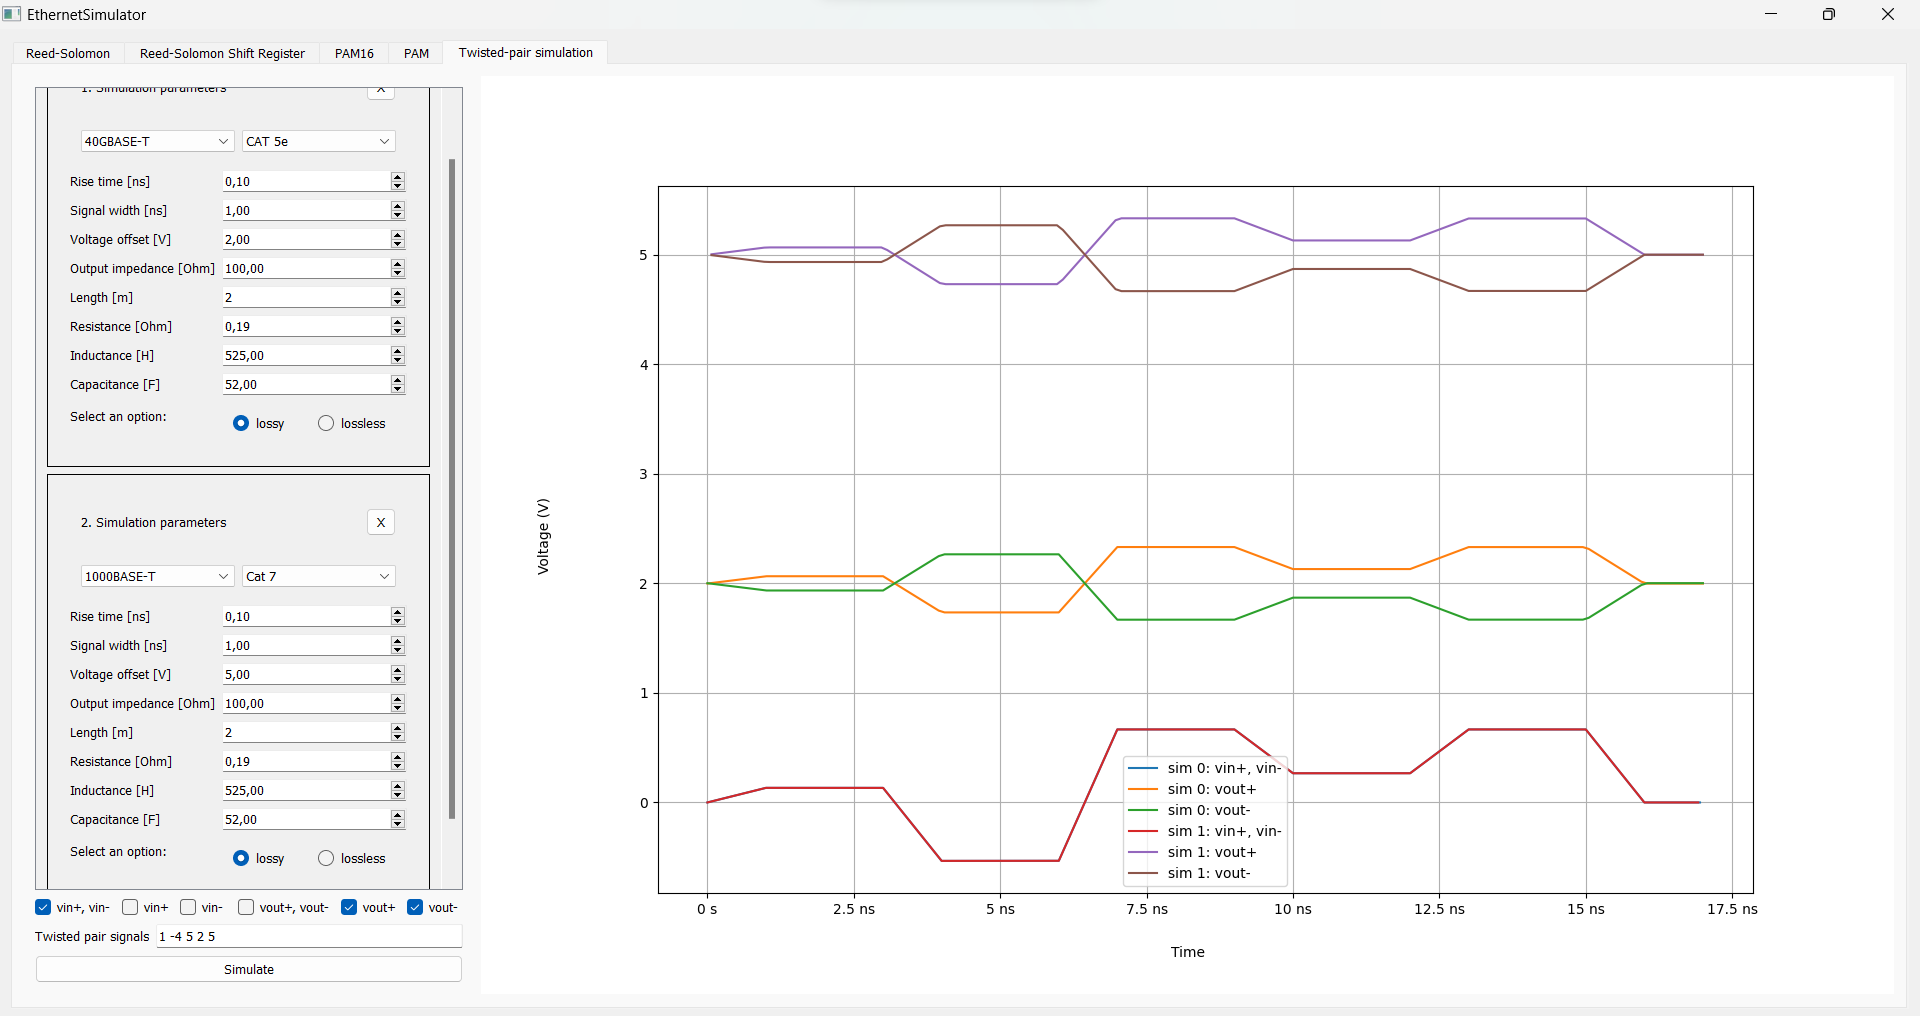
\includegraphics[width=0.95\textwidth]{images/prezentacja_tp.png}
\end{frame}

\end{document}